\documentclass[]{article}
\usepackage{graphicx}
\usepackage{caption}
\usepackage{subcaption}
\newcommand{\ty}[1]{\texttt{#1}}
\begin{document}

\title{COP 290 - Assignment 2\\MyDropbox App}
\author{Akshay Kumar Gupta\\ 2013CS50275 \and  Barun Patra\\{2013CS10773} \and J. Shikhar Murty\\{2013EE10462}}
\date{}
\maketitle
\section{Overall Design}
We have followed a modular design approach with two main classes, \ty{Client} and \ty{Server} along with classes to handle the GUI front end, user authentication, user list and versioning. We have used QT for the front end, C socket API for interprocess communication and OpenSSL for secure data transfer. The major subcomponents of the app are described below.
\section{Client User Interface}
QT has been used to design the front end for the client.
\subsection{Login/Register}
When a user opens the MyDropbox App, he sees a Login/Register page. If he clicks on Register, a form is displayed in which the user enters a username, password and other optional details. The password must be at least 6 characters long and must include at least one uppercase letter, one lowercase letter and one digit. In the Login page, the user enters the username and password. An unsuccessful login keeps the user on the same page with an error message. A successful login takes the user to the main interface.
\subsection{Primary Interface}
After login, the user sees a list of directories and files which he owns or has access to. These are in two sections - the files currently on the user's system and the ones on the server. Internally the file system is a QTTreeWidget. The files on the system have an upload button. This button sends a request to the client middle end with the file path and the file is uploaded to the server. The files in the server section have a download button. Clicking this sends a download request to the middle end with the name of the file and the file is downloaded. While upload/download is under way, a progress bar is shown to the user. There is also an option to delete files that the user owns.
\subsection{Sharing}The user has a share list which shows the files that have been shared with him by other users and the files he has shared with other users. When he wants to share a file with another user he specifies the user's username and then clicks share. He can then set the access permissions to read-only or read/write.
\subsection{Syncing}When the user clicks sync all the files that are currently being edited by the user get uploaded to the server. Moreover, when the user clicks on logout, he is asked whether he wants to sync his changed files. He can thus leave his work on one machine and resume working on another machine.
\begin{figure}
\hspace*{-1.2in}
\begin{subfigure}{.5\textwidth}
 \noindent\makebox[\textwidth]{%
 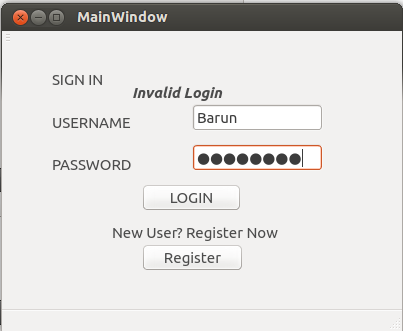
\includegraphics[width=0.7\linewidth]{login.png}}
  \caption{Login Screen}
  \label{fig:sub1}
\end{subfigure}%
\begin{subfigure}{.5\textwidth}
  \centering
  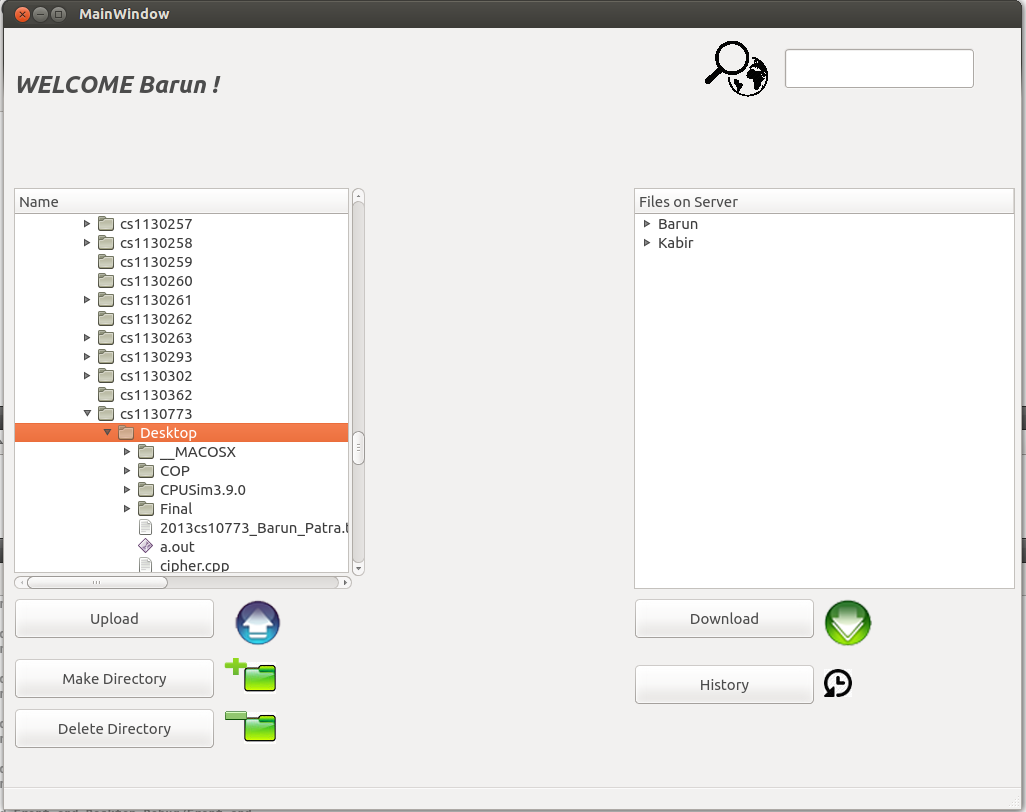
\includegraphics[width=1.8\linewidth]{screen.png}
  \caption{Main Screen}
  \label{fig:sub2}
\end{subfigure}
\caption{User Interface}
\label{fig:test}
\end{figure}
\section{Server Backend}
We have a class called \ty{Server} which handles the server backend. It contains four primary functions:
\begin{itemize}
\item \ty{CreateServer()} - Starts the server and waits for clients to request a connection. We use the socket API in C to communicate between server and client. When a client requests a connection, this function forks into two processes. One process calls \ty{communicateWithClient()} to handle the connected client and the other waits for another client to request a connection. Thus multiple clients can connect to the server at the same time.
\item \ty{communicateWithClient()} - This function handles communication with the client. It receives data from \ty{ReceiveData()}, processes it and sends back data through \ty{SendData()}. The processing is done according to commands sent by \ty{writeToServer()} in the \ty{Client} class.
\item \ty{SignInRequest()} - This function handles the registering and logging in by users. The username and password of the user are hashed into a unique id and stored in a file. When a client logs in this function receives a username and password it checks it against the file and sends back a boolean signal whether or not the credentials are valid.
\item \ty{SendData()} - All the data from server to client is sent through this function. Data is sent over a secure connection. The data can be in different forms:
\begin{itemize}
\item A file : For a file, the name of the file and its length is sent to the client followed by the file contents. This allows the client end to know the extension of the file sent by the server.
\item Request-specific information : Different requests from the user have different responses. The data sent is specific to these requests. For example, a list of versions of a file along with their time stamps, or a list of users using the system etc.
\end{itemize}
\item \ty{ReceiveData()} - All the data from client is received by this function. It reads data from the client which is again either file contents or request-specific information.
\end{itemize}
\section{Client Backend}
We have a class called \ty{Client} which handles the client backend and middle end.
The backend contains the following functions: 
\begin{itemize}
\item \ty{connectToServer()} - This sends a connection request from the client to the server. The client must know the server's IP Address to start a connection. Once a connection is established, the client is ready to send and receive files from server.
\item \ty{readFromServer()} - This reads all the data sent by the server and sends it to the client middle end to parse and process.
\item \ty{writeToServer()} - This receives data from the middle end and send it to the server.  
\end{itemize}
The middle end contains functions corresponding to all the GUI inputs from the user:
\begin{itemize}
\item \ty{register()} - This function receives a username and password. The password is checked against a regular expression to ensure that it is at least 6 characters long and has at least one uppercase character, one lowercase character and one digit. Regex matching is done using the C{}\verb!++! \ty{regex} library. If the password is valid then a string ``Register [username] [password]" is sent to \ty{writeToServer} which sends it to the server.
\item \ty{login()} - This function generates a string ``Login [username] [password]'' which it passes on to \ty{writeToServer()}.
\item \ty{downloadClick()} - This function is executed when the download button next to a particular file is clicked. It generates a string which roughly says ``Download [file path] [version no.]". This is sent to \ty{writeToServer()} which sends this command to the server.
\item \ty{uploadClick()} - When the user clicks upload, a string that says ``Upload [file path]" is sent to \ty{writeToServer()}, which first sends this command to the server followed by the file contents.
\item \ty{share()} - When the user wants to share a file with a user, this function is executed. It sends a string ``Share [file path] [username] [permission]" to \ty{writeToServer()}.
\item \ty{delete()} - This function generates a string ``Delete [file path]'' and sends it to \ty{writeToServer()}.
\item \ty{sync()} - This function generates the string ``Sync [list of files]" and sends it to \ty{writeToServer()}.
\end{itemize}
\section{Security}
The OpenSSL library has been used to securely communicate between the client and the server. The server is not allowed to run unless an authentication certificate has been created. If the certificate exists it is loaded into the \ty{createServer()} function and using this the RSA private and public key for the server machine is generated using OpenSSL. When a client requests a connection, it first receives the certificate from the server. If the certificate is valid, the connection is established.\\ \\ All reads and writes from server to client and vice versa are carried out using \ty{SSL\char`_read()} and \ty{SSL\char`_write()}. The write command encrypts the data using the receiver's public key and the read command decrypts it using the receiver's private key. Hence all communication is carried out securely.
\section{Version Control}
We have a versioning system in which a user has access to all versions of a file that he has previously uploaded to the server.
\subsection{Download request} When a user wants to download a file from the server, he is first shown a list of versions of the file along with their time stamps. He can choose one of these versions and download it and resume working on it.
\subsection{Upload Request} When a user uploads a file the file gets time stamped and is stored as the latest version of that file.
\subsection{Minimal Data Usage}
We use the shell command \ty{diff -e [file1.txt] [file2.txt]} to generate a script of the changes required to convert the first file to the second file. For each upload by the user, we create an edit script to convert the original file to this version of the file. We also time stamp the file. Because we use the \ty{diff} command, minimal amount of extra storage is required to store a version. When a download request is sent by the user, a filename and version number is received by the server backend and we execute the shell command \ty{ed} with the original file and the appropriate edit script. We rely on shell commands for this purpose because they are efficient and reliable.
\section{File Sharing}
\subsection{Share Logs}
Associated with each user, there is a share log file at the server end which records the share history of the user. Each entry has a date and time, a file name, a username, whether the user was given access or gave access to this file and the permission. This allows us to keep track of the entire share history of the user which we can show to him in the user interface.
\subsection{Share Request}
When a user shares a file with another user, the server receives the share command and a new entry is added to both the users' share logs. If the other user is also logged in at the same time, his share list gets updated and he can then see that a file has been shared with him.
\subsection{Access Request}
When a user accesses a file that is shared with him, he receives that file in the same way he would receive a file owned by him. But if the permission for that file is read-only, he will not be allowed to upload an edited file onto the server, even though he can edited it locally.
\section{Persistent Storage}
Our upload/download model also ensures that file storage is persistent. When the user wants to work on a file, he first downloads it from the server. Hence he gets a copy of that file on his local machine. If he loses connection, the local copy will remain on his system, so he does not need to download that file again. When he logs in again, all his local changes are first synced to the server. Hence all changes get saved to the server with minimum pain to the user.
\section{Testing}
We will have test suites for the following subcomponents:
\subsection{User Interface}
\begin{itemize}
\item We will visually check that the user interface displays the correct windows on registration and login and that the main interface is visually correct.
\item We will test that various button clicks invoke the correct functions and that directories and files are shown correctly.
\end{itemize}
\subsection{Security}
We will test that that network is secure by checking that a connection is not allowed to be established unless the server has a valid certificate.
\subsection{Network Connection}
\begin{itemize}
\item We will send connection requests from multiple clients at the same time to check that they can all connect at the same time.
\item We will send a large variety of files of different types and sizes from client to server and vice versa to check that file transfer works correctly.
\item We will then check that different commands like login, share, sync etc. are sent across to the server correctly.
\end{itemize}
\subsection{Server End}
\begin{itemize}
\item We will pass different command strings to the server backend to check whether they are interpreted correctly.
\item We will check that the username and password are hashed uniquely and stored in the file correctly.
\item We will check that share logs are generated correctly and that permissions are handled in a correct way by attempting to upload an edited read-only file.
\end{itemize}
\subsection{Version Control}
We will test that \ty{diff} and \ty{ed} works correctly. We will check that the ratio of actual data stored to the sum of data of all the versions of the file is appropriately small and that it decreases with increase in number of versions. We will test that the correct version in generated when a download request with file name and version is received by the backend.
\subsection{Client End}
We will ensure that all the different middle-end function calls send the correct commands to \ty{writeToServer()} and that the commands are in a correct and unambiguous format. For each command we will create multiple tests which will pass different parameters to each command and check that they are handled correctly.  
\section{Planned Improvements}
\begin{itemize}
\item File Compression : We will compress the files on the server system to further reduce storage memory requirements. For correct versioning, we will generate the edit script for the uncompressed file and then compress the original file and the edit script. We will either use LZW or Burrows-Wheeler Transform for compression.
\item Search bar with autocomplete : Each user will have a search bar to search for names of other users on MyDropbox. This will make it easier for them to search for people to share files with. The search bar will support autocomplete. For fast autocomplete, we will create a ternary search trie (faster variation of a standard trie) with the list of usernames. Each keystroke will be sent to the server which will send back a potential username with that prefix after searching the trie.
\end{itemize}
\end{document}